\documentclass[1p]{elsarticle_modified}
%\bibliographystyle{elsarticle-num}

%\usepackage[colorlinks]{hyperref}
%\usepackage{abbrmath_seonhwa} %\Abb, \Ascr, \Acal ,\Abf, \Afrak
\usepackage{amsfonts}
\usepackage{amssymb}
\usepackage{amsmath}
\usepackage{amsthm}
\usepackage{scalefnt}
\usepackage{amsbsy}
\usepackage{kotex}
\usepackage{caption}
\usepackage{subfig}
\usepackage{color}
\usepackage{graphicx}
\usepackage{xcolor} %% white, black, red, green, blue, cyan, magenta, yellow
\usepackage{float}
\usepackage{setspace}
\usepackage{hyperref}

\usepackage{tikz}
\usetikzlibrary{arrows}

\usepackage{multirow}
\usepackage{array} % fixed length table
\usepackage{hhline}

%%%%%%%%%%%%%%%%%%%%%
\makeatletter
\renewcommand*\env@matrix[1][\arraystretch]{%
	\edef\arraystretch{#1}%
	\hskip -\arraycolsep
	\let\@ifnextchar\new@ifnextchar
	\array{*\c@MaxMatrixCols c}}
\makeatother %https://tex.stackexchange.com/questions/14071/how-can-i-increase-the-line-spacing-in-a-matrix
%%%%%%%%%%%%%%%

\usepackage[normalem]{ulem}

\newcommand{\msout}[1]{\ifmmode\text{\sout{\ensuremath{#1}}}\else\sout{#1}\fi}
%SOURCE: \msout is \stkout macro in https://tex.stackexchange.com/questions/20609/strikeout-in-math-mode

\newcommand{\cancel}[1]{
	\ifmmode
	{\color{red}\msout{#1}}
	\else
	{\color{red}\sout{#1}}
	\fi
}

\newcommand{\add}[1]{
	{\color{blue}\uwave{#1}}
}

\newcommand{\replace}[2]{
	\ifmmode
	{\color{red}\msout{#1}}{\color{blue}\uwave{#2}}
	\else
	{\color{red}\sout{#1}}{\color{blue}\uwave{#2}}
	\fi
}

\newcommand{\Sol}{\mathcal{S}} %segment
\newcommand{\D}{D} %diagram
\newcommand{\A}{\mathcal{A}} %arc


%%%%%%%%%%%%%%%%%%%%%%%%%%%%%5 test

\def\sl{\operatorname{\textup{SL}}(2,\Cbb)}
\def\psl{\operatorname{\textup{PSL}}(2,\Cbb)}
\def\quan{\mkern 1mu \triangleright \mkern 1mu}

\theoremstyle{definition}
\newtheorem{thm}{Theorem}[section]
\newtheorem{prop}[thm]{Proposition}
\newtheorem{lem}[thm]{Lemma}
\newtheorem{ques}[thm]{Question}
\newtheorem{cor}[thm]{Corollary}
\newtheorem{defn}[thm]{Definition}
\newtheorem{exam}[thm]{Example}
\newtheorem{rmk}[thm]{Remark}
\newtheorem{alg}[thm]{Algorithm}

\newcommand{\I}{\sqrt{-1}}
\begin{document}

%\begin{frontmatter}
%
%\title{Boundary parabolic representations of knots up to 8 crossings}
%
%%% Group authors per affiliation:
%\author{Yunhi Cho} 
%\address{Department of Mathematics, University of Seoul, Seoul, Korea}
%\ead{yhcho@uos.ac.kr}
%
%
%\author{Seonhwa Kim} %\fnref{s_kim}}
%\address{Center for Geometry and Physics, Institute for Basic Science, Pohang, 37673, Korea}
%\ead{ryeona17@ibs.re.kr}
%
%\author{Hyuk Kim}
%\address{Department of Mathematical Sciences, Seoul National University, Seoul 08826, Korea}
%\ead{hyukkim@snu.ac.kr}
%
%\author{Seokbeom Yoon}
%\address{Department of Mathematical Sciences, Seoul National University, Seoul, 08826,  Korea}
%\ead{sbyoon15@snu.ac.kr}
%
%\begin{abstract}
%We find all boundary parabolic representation of knots up to 8 crossings.
%
%\end{abstract}
%\begin{keyword}
%    \MSC[2010] 57M25 
%\end{keyword}
%
%\end{frontmatter}

%\linenumbers
%\tableofcontents
%
\newcommand\colored[1]{\textcolor{white}{\rule[-0.35ex]{0.8em}{1.4ex}}\kern-0.8em\color{red} #1}%
%\newcommand\colored[1]{\textcolor{white}{ #1}\kern-2.17ex	\textcolor{white}{ #1}\kern-1.81ex	\textcolor{white}{ #1}\kern-2.15ex\color{red}#1	}

{\Large $\underline{10_{52}~(K10a_{80})}$}

\setlength{\tabcolsep}{10pt}
\renewcommand{\arraystretch}{1.6}
\vspace{1cm}\begin{tabular}{m{100pt}>{\centering\arraybackslash}m{274pt}}
\multirow{5}{120pt}{
	\centering
	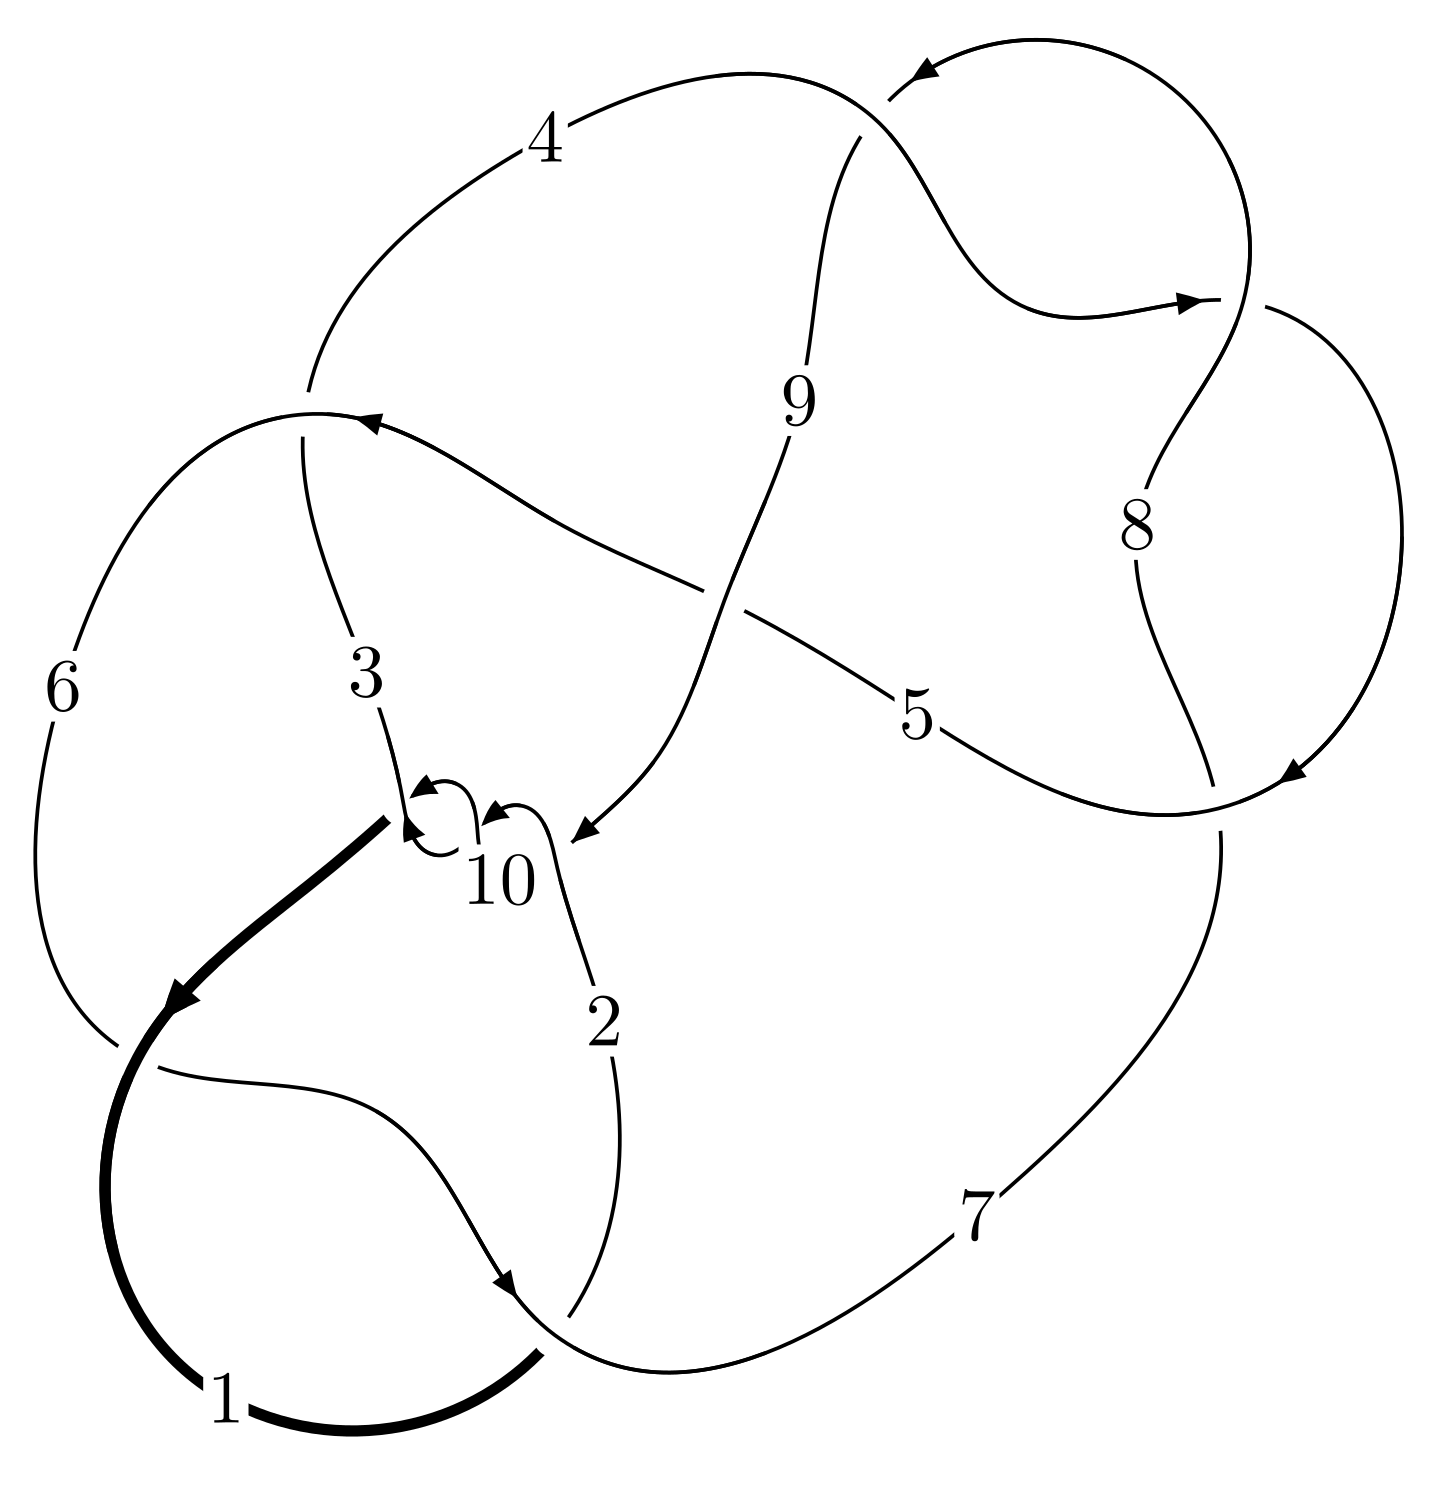
\includegraphics[width=112pt]{../../../GIT/diagram.site/Diagrams/png/136_10_52.png}\\
\ \ \ A knot diagram\footnotemark}&
\allowdisplaybreaks
\textbf{Linearized knot diagam} \\
\cline{2-2}
 &
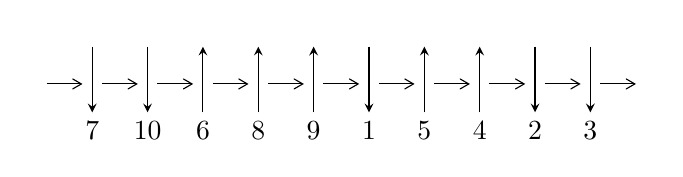
\begin{tikzpicture}[x=20pt, y=17pt]
	% nodes
	\node (C0) at (0, 0) {};
	\node (C1) at (1, 0) {};
	\node (C1U) at (1, +1) {};
	\node (C1D) at (1, -1) {7};

	\node (C2) at (2, 0) {};
	\node (C2U) at (2, +1) {};
	\node (C2D) at (2, -1) {10};

	\node (C3) at (3, 0) {};
	\node (C3U) at (3, +1) {};
	\node (C3D) at (3, -1) {6};

	\node (C4) at (4, 0) {};
	\node (C4U) at (4, +1) {};
	\node (C4D) at (4, -1) {8};

	\node (C5) at (5, 0) {};
	\node (C5U) at (5, +1) {};
	\node (C5D) at (5, -1) {9};

	\node (C6) at (6, 0) {};
	\node (C6U) at (6, +1) {};
	\node (C6D) at (6, -1) {1};

	\node (C7) at (7, 0) {};
	\node (C7U) at (7, +1) {};
	\node (C7D) at (7, -1) {5};

	\node (C8) at (8, 0) {};
	\node (C8U) at (8, +1) {};
	\node (C8D) at (8, -1) {4};

	\node (C9) at (9, 0) {};
	\node (C9U) at (9, +1) {};
	\node (C9D) at (9, -1) {2};

	\node (C10) at (10, 0) {};
	\node (C10U) at (10, +1) {};
	\node (C10D) at (10, -1) {3};
	\node (C11) at (11, 0) {};

	% arrows
	\draw[->,>={angle 60}]
	(C0) edge (C1) (C1) edge (C2) (C2) edge (C3) (C3) edge (C4) (C4) edge (C5) (C5) edge (C6) (C6) edge (C7) (C7) edge (C8) (C8) edge (C9) (C9) edge (C10) (C10) edge (C11) ;	\draw[->,>=stealth]
	(C1U) edge (C1D) (C2U) edge (C2D) (C3D) edge (C3U) (C4D) edge (C4U) (C5D) edge (C5U) (C6U) edge (C6D) (C7D) edge (C7U) (C8D) edge (C8U) (C9U) edge (C9D) (C10U) edge (C10D) ;
	\end{tikzpicture} \\
\hhline{~~} \\& 
\textbf{Solving Sequence} \\ \cline{2-2} 
 &
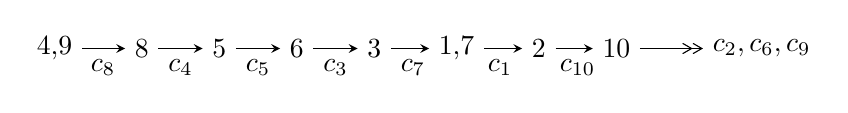
\begin{tikzpicture}[x=28pt, y=7pt]
	% node
	\node (A0) at (-1/8, 0) {4,9};
	\node (A1) at (1, 0) {8};
	\node (A2) at (2, 0) {5};
	\node (A3) at (3, 0) {6};
	\node (A4) at (4, 0) {3};
	\node (A5) at (81/16, 0) {1,7};
	\node (A6) at (49/8, 0) {2};
	\node (A7) at (57/8, 0) {10};
	\node (C1) at (1/2, -1) {$c_{8}$};
	\node (C2) at (3/2, -1) {$c_{4}$};
	\node (C3) at (5/2, -1) {$c_{5}$};
	\node (C4) at (7/2, -1) {$c_{3}$};
	\node (C5) at (9/2, -1) {$c_{7}$};
	\node (C6) at (45/8, -1) {$c_{1}$};
	\node (C7) at (53/8, -1) {$c_{10}$};
	\node (A8) at (9, 0) {$c_{2},c_{6},c_{9}$};

	% edge
	\draw[->,>=stealth]	
	(A0) edge (A1) (A1) edge (A2) (A2) edge (A3) (A3) edge (A4) (A4) edge (A5) (A5) edge (A6) (A6) edge (A7) ;
	\draw[->>,>={angle 60}]	
	(A7) edge (A8);
\end{tikzpicture} \\ 

\end{tabular} \\

\footnotetext{
The image of knot diagram is generated by the software ``\textbf{Draw programme}" developed by Andrew Bartholomew(\url{http://www.layer8.co.uk/maths/draw/index.htm\#Running-draw}), where we modified some parts for our purpose(\url{https://github.com/CATsTAILs/LinksPainter}).
}\phantom \\ \newline 
\centering \textbf{Ideals for irreducible components\footnotemark of $X_{\text{par}}$} 
 
\begin{align*}
I^u_{1}&=\langle 
2 u^{29}+u^{28}+\cdots+b-1,\;u^{31}+2 u^{30}+\cdots+a-3,\;u^{32}+2 u^{31}+\cdots-5 u-1\rangle \\
I^u_{2}&=\langle 
b-1,\;- u^2+a+u-2,\;u^3- u^2+2 u-1\rangle \\
\\
\end{align*}
\raggedright * 2 irreducible components of $\dim_{\mathbb{C}}=0$, with total 35 representations.\\
\footnotetext{All coefficients of polynomials are rational numbers. But the coefficients are sometimes approximated in decimal forms when there is not enough margin.}
\newpage
\renewcommand{\arraystretch}{1}
\centering \section*{I. $I^u_{1}= \langle 2 u^{29}+u^{28}+\cdots+b-1,\;u^{31}+2 u^{30}+\cdots+a-3,\;u^{32}+2 u^{31}+\cdots-5 u-1 \rangle$}
\flushleft \textbf{(i) Arc colorings}\\
\begin{tabular}{m{7pt} m{180pt} m{7pt} m{180pt} }
\flushright $a_{4}=$&$\begin{pmatrix}0\\u\end{pmatrix}$ \\
\flushright $a_{9}=$&$\begin{pmatrix}1\\0\end{pmatrix}$ \\
\flushright $a_{8}=$&$\begin{pmatrix}1\\u^2\end{pmatrix}$ \\
\flushright $a_{5}=$&$\begin{pmatrix}u\\u^3+u\end{pmatrix}$ \\
\flushright $a_{6}=$&$\begin{pmatrix}u^3+2 u\\u^3+u\end{pmatrix}$ \\
\flushright $a_{3}=$&$\begin{pmatrix}- u^7-4 u^5-4 u^3\\- u^7-3 u^5-2 u^3+u\end{pmatrix}$ \\
\flushright $a_{1}=$&$\begin{pmatrix}- u^{31}-2 u^{30}+\cdots+u+3\\-2 u^{29}- u^{28}+\cdots+2 u+1\end{pmatrix}$ \\
\flushright $a_{7}=$&$\begin{pmatrix}u^2+1\\u^4+2 u^2\end{pmatrix}$ \\
\flushright $a_{2}=$&$\begin{pmatrix}- u^{31}-2 u^{30}+\cdots+6 u+4\\- u^{29}- u^{28}+\cdots+u+1\end{pmatrix}$ \\
\flushright $a_{10}=$&$\begin{pmatrix}- u^{31}-2 u^{30}+\cdots+4 u+4\\- u^{29}- u^{28}+\cdots+2 u+1\end{pmatrix}$\\&\end{tabular}
\flushleft \textbf{(ii) Obstruction class $= -1$}\\~\\
\flushleft \textbf{(iii) Cusp Shapes $= u^{31}+2 u^{30}+16 u^{29}+30 u^{28}+116 u^{27}+201 u^{26}+500 u^{25}+783 u^{24}+1406 u^{23}+1926 u^{22}+2640 u^{21}+3005 u^{20}+3188 u^{19}+2713 u^{18}+2078 u^{17}+811 u^{16}+52 u^{15}-886 u^{14}-904 u^{13}-890 u^{12}-388 u^{11}-158 u^{10}+98 u^9-10 u^7-104 u^6-38 u^5-21 u^4+42 u^3+21 u^2+6 u-9$}\\~\\
\newpage\renewcommand{\arraystretch}{1}
\flushleft \textbf{(iv) u-Polynomials at the component}\newline \\
\begin{tabular}{m{50pt}|m{274pt}}
Crossings & \hspace{64pt}u-Polynomials at each crossing \\
\hline $$\begin{aligned}c_{1},c_{6}\end{aligned}$$&$\begin{aligned}
&u^{32}- u^{31}+\cdots+4 u+8
\end{aligned}$\\
\hline $$\begin{aligned}c_{2},c_{9},c_{10}\end{aligned}$$&$\begin{aligned}
&u^{32}-4 u^{31}+\cdots+2 u-1
\end{aligned}$\\
\hline $$\begin{aligned}c_{3}\end{aligned}$$&$\begin{aligned}
&u^{32}+6 u^{31}+\cdots-29 u+19
\end{aligned}$\\
\hline $$\begin{aligned}c_{4},c_{7},c_{8}\end{aligned}$$&$\begin{aligned}
&u^{32}+2 u^{31}+\cdots-5 u-1
\end{aligned}$\\
\hline $$\begin{aligned}c_{5}\end{aligned}$$&$\begin{aligned}
&u^{32}-2 u^{31}+\cdots-91 u-17
\end{aligned}$\\
\hline
\end{tabular}\\~\\
\newpage\renewcommand{\arraystretch}{1}
\flushleft \textbf{(v) Riley Polynomials at the component}\newline \\
\begin{tabular}{m{50pt}|m{274pt}}
Crossings & \hspace{64pt}Riley Polynomials at each crossing \\
\hline $$\begin{aligned}c_{1},c_{6}\end{aligned}$$&$\begin{aligned}
&y^{32}-21 y^{31}+\cdots-400 y+64
\end{aligned}$\\
\hline $$\begin{aligned}c_{2},c_{9},c_{10}\end{aligned}$$&$\begin{aligned}
&y^{32}-32 y^{31}+\cdots+10 y+1
\end{aligned}$\\
\hline $$\begin{aligned}c_{3}\end{aligned}$$&$\begin{aligned}
&y^{32}+18 y^{31}+\cdots-14597 y+361
\end{aligned}$\\
\hline $$\begin{aligned}c_{4},c_{7},c_{8}\end{aligned}$$&$\begin{aligned}
&y^{32}+30 y^{31}+\cdots-17 y+1
\end{aligned}$\\
\hline $$\begin{aligned}c_{5}\end{aligned}$$&$\begin{aligned}
&y^{32}+6 y^{31}+\cdots-2025 y+289
\end{aligned}$\\
\hline
\end{tabular}\\~\\
\newpage\flushleft \textbf{(vi) Complex Volumes and Cusp Shapes}
$$\begin{array}{c|c|c}  
\text{Solutions to }I^u_{1}& \I (\text{vol} + \sqrt{-1}CS) & \text{Cusp shape}\\
 \hline 
\begin{aligned}
u &= -0.533924 + 0.635384 I \\
a &= -1.44678 + 1.16510 I \\
b &= -0.03219 + 1.54133 I\end{aligned}
 & -8.33717 + 3.47045 I & -6.19300 - 0.53804 I \\ \hline\begin{aligned}
u &= -0.533924 - 0.635384 I \\
a &= -1.44678 - 1.16510 I \\
b &= -0.03219 - 1.54133 I\end{aligned}
 & -8.33717 - 3.47045 I & -6.19300 + 0.53804 I \\ \hline\begin{aligned}
u &= -0.737398 + 0.363177 I \\
a &= \phantom{-}1.39466 - 1.92116 I \\
b &= \phantom{-}0.33070 - 1.92317 I\end{aligned}
 & -7.36935 - 7.82848 I & -4.18330 + 6.10894 I \\ \hline\begin{aligned}
u &= -0.737398 - 0.363177 I \\
a &= \phantom{-}1.39466 + 1.92116 I \\
b &= \phantom{-}0.33070 + 1.92317 I\end{aligned}
 & -7.36935 + 7.82848 I & -4.18330 - 6.10894 I \\ \hline\begin{aligned}
u &= \phantom{-}0.121416 + 1.191480 I \\
a &= \phantom{-}0.222642 - 0.520130 I \\
b &= -0.646759 - 0.202123 I\end{aligned}
 & -1.84659 + 2.03195 I & -0.06352 - 4.09496 I \\ \hline\begin{aligned}
u &= \phantom{-}0.121416 - 1.191480 I \\
a &= \phantom{-}0.222642 + 0.520130 I \\
b &= -0.646759 + 0.202123 I\end{aligned}
 & -1.84659 - 2.03195 I & -0.06352 + 4.09496 I \\ \hline\begin{aligned}
u &= \phantom{-}0.772369\phantom{ +0.000000I} \\
a &= -0.383393\phantom{ +0.000000I} \\
b &= \phantom{-}0.296121\phantom{ +0.000000I}\end{aligned}
 & -2.56303\phantom{ +0.000000I} & -3.36180\phantom{ +0.000000I} \\ \hline\begin{aligned}
u &= \phantom{-}0.321817 + 1.204360 I \\
a &= -0.378231 + 0.177725 I \\
b &= \phantom{-}0.335766 + 0.398330 I\end{aligned}
 & -6.26853 + 3.96490 I & -7.15642 - 4.13069 I \\ \hline\begin{aligned}
u &= \phantom{-}0.321817 - 1.204360 I \\
a &= -0.378231 - 0.177725 I \\
b &= \phantom{-}0.335766 - 0.398330 I\end{aligned}
 & -6.26853 - 3.96490 I & -7.15642 + 4.13069 I \\ \hline\begin{aligned}
u &= -0.046033 + 1.276630 I \\
a &= \phantom{-}0.169895 + 1.097880 I \\
b &= \phantom{-}1.40941 - 0.16635 I\end{aligned}
 & -4.89788 - 1.11555 I & -6.11098 - 0.26189 I\\
 \hline 
 \end{array}$$\newpage$$\begin{array}{c|c|c}  
\text{Solutions to }I^u_{1}& \I (\text{vol} + \sqrt{-1}CS) & \text{Cusp shape}\\
 \hline 
\begin{aligned}
u &= -0.046033 - 1.276630 I \\
a &= \phantom{-}0.169895 - 1.097880 I \\
b &= \phantom{-}1.40941 + 0.16635 I\end{aligned}
 & -4.89788 + 1.11555 I & -6.11098 + 0.26189 I \\ \hline\begin{aligned}
u &= -0.637579 + 0.336310 I \\
a &= -1.77319 + 1.89857 I \\
b &= -0.49204 + 1.80683 I\end{aligned}
 & -1.10997 - 4.05552 I & -1.42840 + 6.80075 I \\ \hline\begin{aligned}
u &= -0.637579 - 0.336310 I \\
a &= -1.77319 - 1.89857 I \\
b &= -0.49204 - 1.80683 I\end{aligned}
 & -1.10997 + 4.05552 I & -1.42840 - 6.80075 I \\ \hline\begin{aligned}
u &= \phantom{-}0.573185 + 0.380549 I \\
a &= -0.567444 - 0.158963 I \\
b &= \phantom{-}0.264757 + 0.307056 I\end{aligned}
 & -3.48280 + 1.78898 I & -3.34736 - 3.66370 I \\ \hline\begin{aligned}
u &= \phantom{-}0.573185 - 0.380549 I \\
a &= -0.567444 + 0.158963 I \\
b &= \phantom{-}0.264757 - 0.307056 I\end{aligned}
 & -3.48280 - 1.78898 I & -3.34736 + 3.66370 I \\ \hline\begin{aligned}
u &= \phantom{-}0.214793 + 1.351600 I \\
a &= \phantom{-}0.225799 + 0.123979 I \\
b &= \phantom{-}0.119070 - 0.331821 I\end{aligned}
 & -3.45767 + 3.36417 I & \phantom{-}0.37870 - 3.50479 I \\ \hline\begin{aligned}
u &= \phantom{-}0.214793 - 1.351600 I \\
a &= \phantom{-}0.225799 - 0.123979 I \\
b &= \phantom{-}0.119070 + 0.331821 I\end{aligned}
 & -3.45767 - 3.36417 I & \phantom{-}0.37870 + 3.50479 I \\ \hline\begin{aligned}
u &= -0.457656 + 0.423798 I \\
a &= \phantom{-}1.94595 - 1.20331 I \\
b &= \phantom{-}0.38062 - 1.37539 I\end{aligned}
 & -1.72217 + 0.51232 I & -4.14141 + 0.14369 I \\ \hline\begin{aligned}
u &= -0.457656 - 0.423798 I \\
a &= \phantom{-}1.94595 + 1.20331 I \\
b &= \phantom{-}0.38062 + 1.37539 I\end{aligned}
 & -1.72217 - 0.51232 I & -4.14141 - 0.14369 I \\ \hline\begin{aligned}
u &= \phantom{-}0.569557 + 0.125662 I \\
a &= \phantom{-}0.316122 + 0.218549 I \\
b &= -0.152586 - 0.164201 I\end{aligned}
 & \phantom{-}1.244440 + 0.519638 I & \phantom{-}6.41959 - 1.56914 I\\
 \hline 
 \end{array}$$\newpage$$\begin{array}{c|c|c}  
\text{Solutions to }I^u_{1}& \I (\text{vol} + \sqrt{-1}CS) & \text{Cusp shape}\\
 \hline 
\begin{aligned}
u &= \phantom{-}0.569557 - 0.125662 I \\
a &= \phantom{-}0.316122 - 0.218549 I \\
b &= -0.152586 + 0.164201 I\end{aligned}
 & \phantom{-}1.244440 - 0.519638 I & \phantom{-}6.41959 + 1.56914 I \\ \hline\begin{aligned}
u &= -0.19027 + 1.43367 I \\
a &= \phantom{-}1.50108 + 0.51525 I \\
b &= \phantom{-}1.02431 - 2.05401 I\end{aligned}
 & -7.59173 - 1.96238 I & -7.59391 + 0. I\phantom{ +0.000000I} \\ \hline\begin{aligned}
u &= -0.19027 - 1.43367 I \\
a &= \phantom{-}1.50108 - 0.51525 I \\
b &= \phantom{-}1.02431 + 2.05401 I\end{aligned}
 & -7.59173 + 1.96238 I & -7.59391 + 0. I\phantom{ +0.000000I} \\ \hline\begin{aligned}
u &= -0.24454 + 1.43301 I \\
a &= -1.68707 - 0.19420 I \\
b &= -0.69085 + 2.37010 I\end{aligned}
 & -6.78693 - 7.28997 I & -5.63030 + 6.08966 I \\ \hline\begin{aligned}
u &= -0.24454 - 1.43301 I \\
a &= -1.68707 + 0.19420 I \\
b &= -0.69085 - 2.37010 I\end{aligned}
 & -6.78693 + 7.28997 I & -5.63030 - 6.08966 I \\ \hline\begin{aligned}
u &= \phantom{-}0.21981 + 1.44034 I \\
a &= -0.396703 - 0.147942 I \\
b &= -0.125890 + 0.603905 I\end{aligned}
 & -9.32026 + 4.72345 I & -7.29654 - 3.13438 I \\ \hline\begin{aligned}
u &= \phantom{-}0.21981 - 1.44034 I \\
a &= -0.396703 + 0.147942 I \\
b &= -0.125890 - 0.603905 I\end{aligned}
 & -9.32026 - 4.72345 I & -7.29654 + 3.13438 I \\ \hline\begin{aligned}
u &= -0.28148 + 1.45411 I \\
a &= \phantom{-}1.58198 - 0.01901 I \\
b &= \phantom{-}0.41766 - 2.30572 I\end{aligned}
 & -13.2076 - 11.5375 I & -7.79347 + 6.25344 I \\ \hline\begin{aligned}
u &= -0.28148 - 1.45411 I \\
a &= \phantom{-}1.58198 + 0.01901 I \\
b &= \phantom{-}0.41766 + 2.30572 I\end{aligned}
 & -13.2076 + 11.5375 I & -7.79347 - 6.25344 I \\ \hline\begin{aligned}
u &= -0.14244 + 1.49315 I \\
a &= -1.134180 - 0.397538 I \\
b &= -0.75514 + 1.63687 I\end{aligned}
 & -15.2480 + 1.1861 I & -9.66994 + 0. I\phantom{ +0.000000I}\\
 \hline 
 \end{array}$$\newpage$$\begin{array}{c|c|c}  
\text{Solutions to }I^u_{1}& \I (\text{vol} + \sqrt{-1}CS) & \text{Cusp shape}\\
 \hline 
\begin{aligned}
u &= -0.14244 - 1.49315 I \\
a &= -1.134180 + 0.397538 I \\
b &= -0.75514 - 1.63687 I\end{aligned}
 & -15.2480 - 1.1861 I & -9.66994 + 0. I\phantom{ +0.000000I} \\ \hline\begin{aligned}
u &= -0.270853\phantom{ +0.000000I} \\
a &= \phantom{-}3.43431\phantom{ +0.000000I} \\
b &= \phantom{-}0.930194\phantom{ +0.000000I}\end{aligned}
 & -1.22025\phantom{ +0.000000I} & -10.0180\phantom{ +0.000000I}\\
 \hline 
 \end{array}$$\newpage\newpage\renewcommand{\arraystretch}{1}
\centering \section*{II. $I^u_{2}= \langle b-1,\;- u^2+a+u-2,\;u^3- u^2+2 u-1 \rangle$}
\flushleft \textbf{(i) Arc colorings}\\
\begin{tabular}{m{7pt} m{180pt} m{7pt} m{180pt} }
\flushright $a_{4}=$&$\begin{pmatrix}0\\u\end{pmatrix}$ \\
\flushright $a_{9}=$&$\begin{pmatrix}1\\0\end{pmatrix}$ \\
\flushright $a_{8}=$&$\begin{pmatrix}1\\u^2\end{pmatrix}$ \\
\flushright $a_{5}=$&$\begin{pmatrix}u\\u^2- u+1\end{pmatrix}$ \\
\flushright $a_{6}=$&$\begin{pmatrix}u^2+1\\u^2- u+1\end{pmatrix}$ \\
\flushright $a_{3}=$&$\begin{pmatrix}-1\\0\end{pmatrix}$ \\
\flushright $a_{1}=$&$\begin{pmatrix}u^2- u+2\\1\end{pmatrix}$ \\
\flushright $a_{7}=$&$\begin{pmatrix}u^2+1\\u^2- u+1\end{pmatrix}$ \\
\flushright $a_{2}=$&$\begin{pmatrix}u^2- u+2\\1\end{pmatrix}$ \\
\flushright $a_{10}=$&$\begin{pmatrix}u^2- u+3\\1\end{pmatrix}$\\&\end{tabular}
\flushleft \textbf{(ii) Obstruction class $= 1$}\\~\\
\flushleft \textbf{(iii) Cusp Shapes $= 5 u^2-4 u+4$}\\~\\
\newpage\renewcommand{\arraystretch}{1}
\flushleft \textbf{(iv) u-Polynomials at the component}\newline \\
\begin{tabular}{m{50pt}|m{274pt}}
Crossings & \hspace{64pt}u-Polynomials at each crossing \\
\hline $$\begin{aligned}c_{1},c_{6}\end{aligned}$$&$\begin{aligned}
&u^3
\end{aligned}$\\
\hline $$\begin{aligned}c_{2}\end{aligned}$$&$\begin{aligned}
&(u+1)^3
\end{aligned}$\\
\hline $$\begin{aligned}c_{3},c_{5}\end{aligned}$$&$\begin{aligned}
&u^3- u^2+1
\end{aligned}$\\
\hline $$\begin{aligned}c_{4}\end{aligned}$$&$\begin{aligned}
&u^3+u^2+2 u+1
\end{aligned}$\\
\hline $$\begin{aligned}c_{7},c_{8}\end{aligned}$$&$\begin{aligned}
&u^3- u^2+2 u-1
\end{aligned}$\\
\hline $$\begin{aligned}c_{9},c_{10}\end{aligned}$$&$\begin{aligned}
&(u-1)^3
\end{aligned}$\\
\hline
\end{tabular}\\~\\
\newpage\renewcommand{\arraystretch}{1}
\flushleft \textbf{(v) Riley Polynomials at the component}\newline \\
\begin{tabular}{m{50pt}|m{274pt}}
Crossings & \hspace{64pt}Riley Polynomials at each crossing \\
\hline $$\begin{aligned}c_{1},c_{6}\end{aligned}$$&$\begin{aligned}
&y^3
\end{aligned}$\\
\hline $$\begin{aligned}c_{2},c_{9},c_{10}\end{aligned}$$&$\begin{aligned}
&(y-1)^3
\end{aligned}$\\
\hline $$\begin{aligned}c_{3},c_{5}\end{aligned}$$&$\begin{aligned}
&y^3- y^2+2 y-1
\end{aligned}$\\
\hline $$\begin{aligned}c_{4},c_{7},c_{8}\end{aligned}$$&$\begin{aligned}
&y^3+3 y^2+2 y-1
\end{aligned}$\\
\hline
\end{tabular}\\~\\
\newpage\flushleft \textbf{(vi) Complex Volumes and Cusp Shapes}
$$\begin{array}{c|c|c}  
\text{Solutions to }I^u_{2}& \I (\text{vol} + \sqrt{-1}CS) & \text{Cusp shape}\\
 \hline 
\begin{aligned}
u &= \phantom{-}0.215080 + 1.307140 I \\
a &= \phantom{-}0.122561 - 0.744862 I \\
b &= \phantom{-}1.00000\phantom{ +0.000000I}\end{aligned}
 & -4.66906 + 2.82812 I & -5.17211 - 2.41717 I \\ \hline\begin{aligned}
u &= \phantom{-}0.215080 - 1.307140 I \\
a &= \phantom{-}0.122561 + 0.744862 I \\
b &= \phantom{-}1.00000\phantom{ +0.000000I}\end{aligned}
 & -4.66906 - 2.82812 I & -5.17211 + 2.41717 I \\ \hline\begin{aligned}
u &= \phantom{-}0.569840\phantom{ +0.000000I} \\
a &= \phantom{-}1.75488\phantom{ +0.000000I} \\
b &= \phantom{-}1.00000\phantom{ +0.000000I}\end{aligned}
 & -0.531480\phantom{ +0.000000I} & \phantom{-}3.34420\phantom{ +0.000000I}\\
 \hline 
 \end{array}$$\newpage
\newpage\renewcommand{\arraystretch}{1}
\centering \section*{ III. u-Polynomials}
\begin{tabular}{m{50pt}|m{274pt}}
Crossings & \hspace{64pt}u-Polynomials at each crossing \\
\hline $$\begin{aligned}c_{1},c_{6}\end{aligned}$$&$\begin{aligned}
&u^3(u^{32}- u^{31}+\cdots+4 u+8)
\end{aligned}$\\
\hline $$\begin{aligned}c_{2}\end{aligned}$$&$\begin{aligned}
&((u+1)^3)(u^{32}-4 u^{31}+\cdots+2 u-1)
\end{aligned}$\\
\hline $$\begin{aligned}c_{3}\end{aligned}$$&$\begin{aligned}
&(u^3- u^2+1)(u^{32}+6 u^{31}+\cdots-29 u+19)
\end{aligned}$\\
\hline $$\begin{aligned}c_{4}\end{aligned}$$&$\begin{aligned}
&(u^3+u^2+2 u+1)(u^{32}+2 u^{31}+\cdots-5 u-1)
\end{aligned}$\\
\hline $$\begin{aligned}c_{5}\end{aligned}$$&$\begin{aligned}
&(u^3- u^2+1)(u^{32}-2 u^{31}+\cdots-91 u-17)
\end{aligned}$\\
\hline $$\begin{aligned}c_{7},c_{8}\end{aligned}$$&$\begin{aligned}
&(u^3- u^2+2 u-1)(u^{32}+2 u^{31}+\cdots-5 u-1)
\end{aligned}$\\
\hline $$\begin{aligned}c_{9},c_{10}\end{aligned}$$&$\begin{aligned}
&((u-1)^3)(u^{32}-4 u^{31}+\cdots+2 u-1)
\end{aligned}$\\
\hline
\end{tabular}\newpage\renewcommand{\arraystretch}{1}
\centering \section*{ IV. Riley Polynomials}
\begin{tabular}{m{50pt}|m{274pt}}
Crossings & \hspace{64pt}Riley Polynomials at each crossing \\
\hline $$\begin{aligned}c_{1},c_{6}\end{aligned}$$&$\begin{aligned}
&y^3(y^{32}-21 y^{31}+\cdots-400 y+64)
\end{aligned}$\\
\hline $$\begin{aligned}c_{2},c_{9},c_{10}\end{aligned}$$&$\begin{aligned}
&((y-1)^3)(y^{32}-32 y^{31}+\cdots+10 y+1)
\end{aligned}$\\
\hline $$\begin{aligned}c_{3}\end{aligned}$$&$\begin{aligned}
&(y^3- y^2+2 y-1)(y^{32}+18 y^{31}+\cdots-14597 y+361)
\end{aligned}$\\
\hline $$\begin{aligned}c_{4},c_{7},c_{8}\end{aligned}$$&$\begin{aligned}
&(y^3+3 y^2+2 y-1)(y^{32}+30 y^{31}+\cdots-17 y+1)
\end{aligned}$\\
\hline $$\begin{aligned}c_{5}\end{aligned}$$&$\begin{aligned}
&(y^3- y^2+2 y-1)(y^{32}+6 y^{31}+\cdots-2025 y+289)
\end{aligned}$\\
\hline
\end{tabular}
\vskip 2pc
\end{document}